\documentclass{article}

\usepackage[utf8]{inputenc}
\usepackage{amsmath}
\usepackage{amsfonts}
\usepackage{amssymb}
\usepackage{graphicx}
\usepackage[table,xcdraw]{xcolor}
\usepackage[hidelinks]{hyperref}
\usepackage{fontawesome5}
\usepackage{longtable}


\graphicspath{ {./images/} }

\renewcommand{\contentsname}{Indice}

\makeatletter
\newcommand*{\rom}[1]{\expandafter\@slowromancap\romannumeral #1@}
\makeatother

\usepackage[a4paper,top=2cm,bottom=2cm,left=2cm,right=2cm]{geometry}


\title{\textbf{\Huge Documento di Architettura}}
\author{Edoardo Ghirardello, Giulio Cappelli, Elia Casotti \\ \\ Gruppo T42}
\date{2022}

\let\origthesubsection\thesubsection

\begin{document}

\maketitle

\clearpage
\tableofcontents
\clearpage

\section{Scopo del documento}
\begin{description}
    \item[] Nel presente documento viene definita l'architettura del sistema "Fen Festa" utilizzando il Class Diagram UML e codice in OCL (Object Constraint Language). \\
        Nel precedente documento sono stati rappresentati i componenti del sistema che ora verranno tradotti in classi attraverso il diagramma UML indicato.
\end{description}
\clearpage
\section{Diagramma delle Classi}
\begin{description}
    \item[] Nel presente capitolo vengono rappresentate le classi previste nell'ambito del progetto "Fen Festa". Ogni componente presente nel diagramma dei componenti diventa una classe. Tutte le classi individuate sono caratterizzate da un nome, una lista di attributi e una lista di metodi che definiscono le operazioni previste all’interno della classe. Associazioni tra le diverse classi forniscono informazioni sulle relazioni tra esse. \\
        Riportiamo di seguito le classi individuate.
\end{description}
\subsection{Utenti}
\begin{description}
    \item[] Analizzando il diagramma di contesto e quello dei componenti si individua la presenza di diversi attori per definire diversi lielli di "User". In particolare si identificano lo user non autenticato \textbf{UtenteNonRegistrato} da cui deriva quello autenticato \textbf{Utente} e i due da esso derivati \textbf{Organizzatore} e \textbf{Admin}.
    \item[] \textbf{Utente} è colui che utlizza l'app per vedere gli eventi disponibili, abbia esso effettuato il login o meno (il login offre più funzionalità specificate in documenti precedenti che verranno meglio identificate successivamente nella seizone inerente OCL).
    \item[] \textbf{Organizzatore} e \textbf{Admin} sono due tipi specifici di utente che dispongono di autorizzazioni extra, sono quindi classi derivate tramite generalizzazione dalla classe \textbf{Utente}
\end{description}
\begin{center}
    \item[] 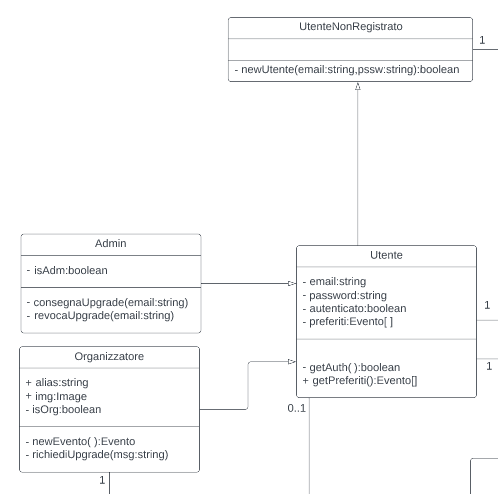
\includegraphics[scale=0.7]{utenti.png}
\end{center}
\newpage
\subsection{Gestione Autenticazione e Account}
\begin{description}
    \item[] Il diagramma dei componenti include diversi componenti per la gestione degli account a partire dalla creazione di un nuovo account, passando dall'autenticazione e permettendo la gestione del proprio account. Definiamo quindi le classi \textbf{CreazioneAccount}, \textbf{GestoreAutenticazione} e \textbf{GestoreAccount}. La classe \textbf{CreazioneAccount} viene utilizzato unicamente dall'utente non ancora registrato, permettendo poi all'utente di autenticarsi. Il \textbf{GestoreAccount} presenta diversi metodi usati sia da utenti normali che da Admin e Organizzatori con l'autorizzazione specifica.
\end{description}
\begin{center}
    \item[] 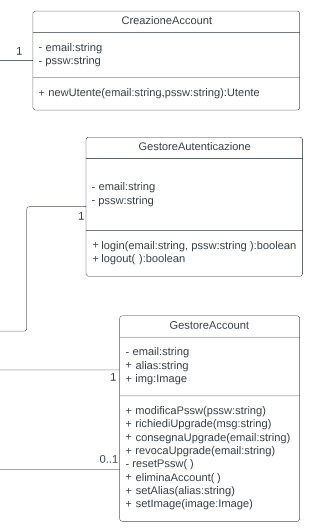
\includegraphics[scale=0.7]{account.png}
\end{center}
\newpage
\subsection{Creazione e Gestione Eventi}
\begin{description}
    \item[] Il diagramma dei componenti identifica due componenti per la gestione degli eventi, dividendo il processo in una prima parte di creazione e una seconda di gestione. Avendo accesso all'intero elenco di eventi la gestione si occupa anche di effettuare la ricerca di un evento. Vengono quindi identificate le rispettive classi \textbf{CreazioneEventi} \textbf{GestoreEventi}.
\end{description}
\begin{center}
    \item[] 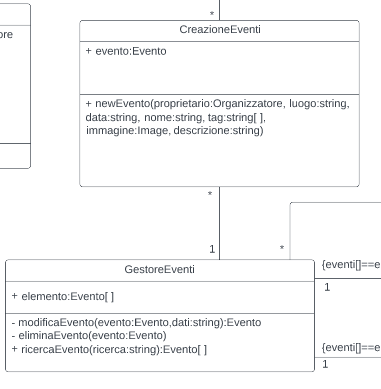
\includegraphics[scale=0.7]{gestoreEventi.png}
\end{center}
\subsection{Visualizzazione degli eventi}
\begin{description}
    \item[] Il diagramma dei componenti identifica i componenti \textbf{Gestore Visualizzazione Evento}, \textbf{Mappa} e \textbf{Elenco Eventi} che assieme si occupano di mostrare agli utenti gli eventi. Creando una classe per ogni componente identifichiamo \textbf{Mappa}, \textbf{ElencoEventi} e \textbf{GestoreVisualizzazioneEvento}. L'utente si interfaccia con queste classi per ricercare e visualizzare gli eventi salvati in app. Può visualizzare i dati del dingolo evento mostrati dal \textbf{GestoreVisualizzazioneEvento}.
\end{description}
\begin{center}
    \item[] 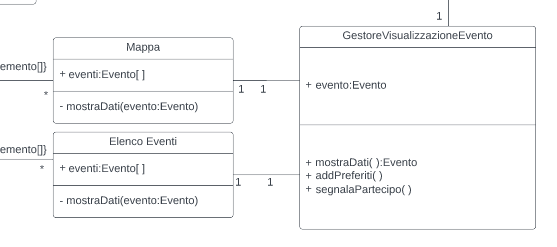
\includegraphics[scale=0.7]{visualizzaEventi.png}
\end{center}
\newpage
\subsection{Gestione Preferiti}
\begin{description}
    \item[] Il diagramma dei componenti identifica un gestore dei preferiti per permettere all'utente autenticato di salvarsi gli eventi a cui è interessato. Identifichiamo quindi la classe \textbf{GestorePreferiti}.
\end{description}
\begin{center}
    \item[] 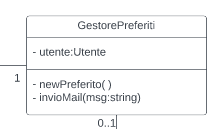
\includegraphics[scale=0.7]{preferiti.png}
\end{center}
\subsection{Gestione Notifiche}
\begin{description}
    \item[] Il diagramma dei componenti identifica un gestore delle notifiche che si occupa dell'invio di email per il recupero della password e per notificare l'utente autenticato dei suoi eventi preferiti. Identifichiamo la classe \textbf{GestoreNotifiche} per gestire questi messaggi in base alle richieste che riceve dal \textbf{GestorePreferiti} e dal \textbf{GestoreAccount}.
\end{description}
\begin{center}
    \item[] 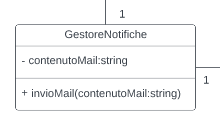
\includegraphics[scale=0.7]{notifiche.png}
\end{center}
\newpage
\subsection{Diagramma delle Classi Complessivo}
\begin{description}
    \item[] Riportiamo di seguito il diagramma delle classi con tutte le classi presentate. È presente inoltre una classe ausiliaria, "Evento", per descrivere il tipo di dato "Evento" utilizzato da altre classi nel diagramma.
\end{description}
\begin{center}
    \item[] 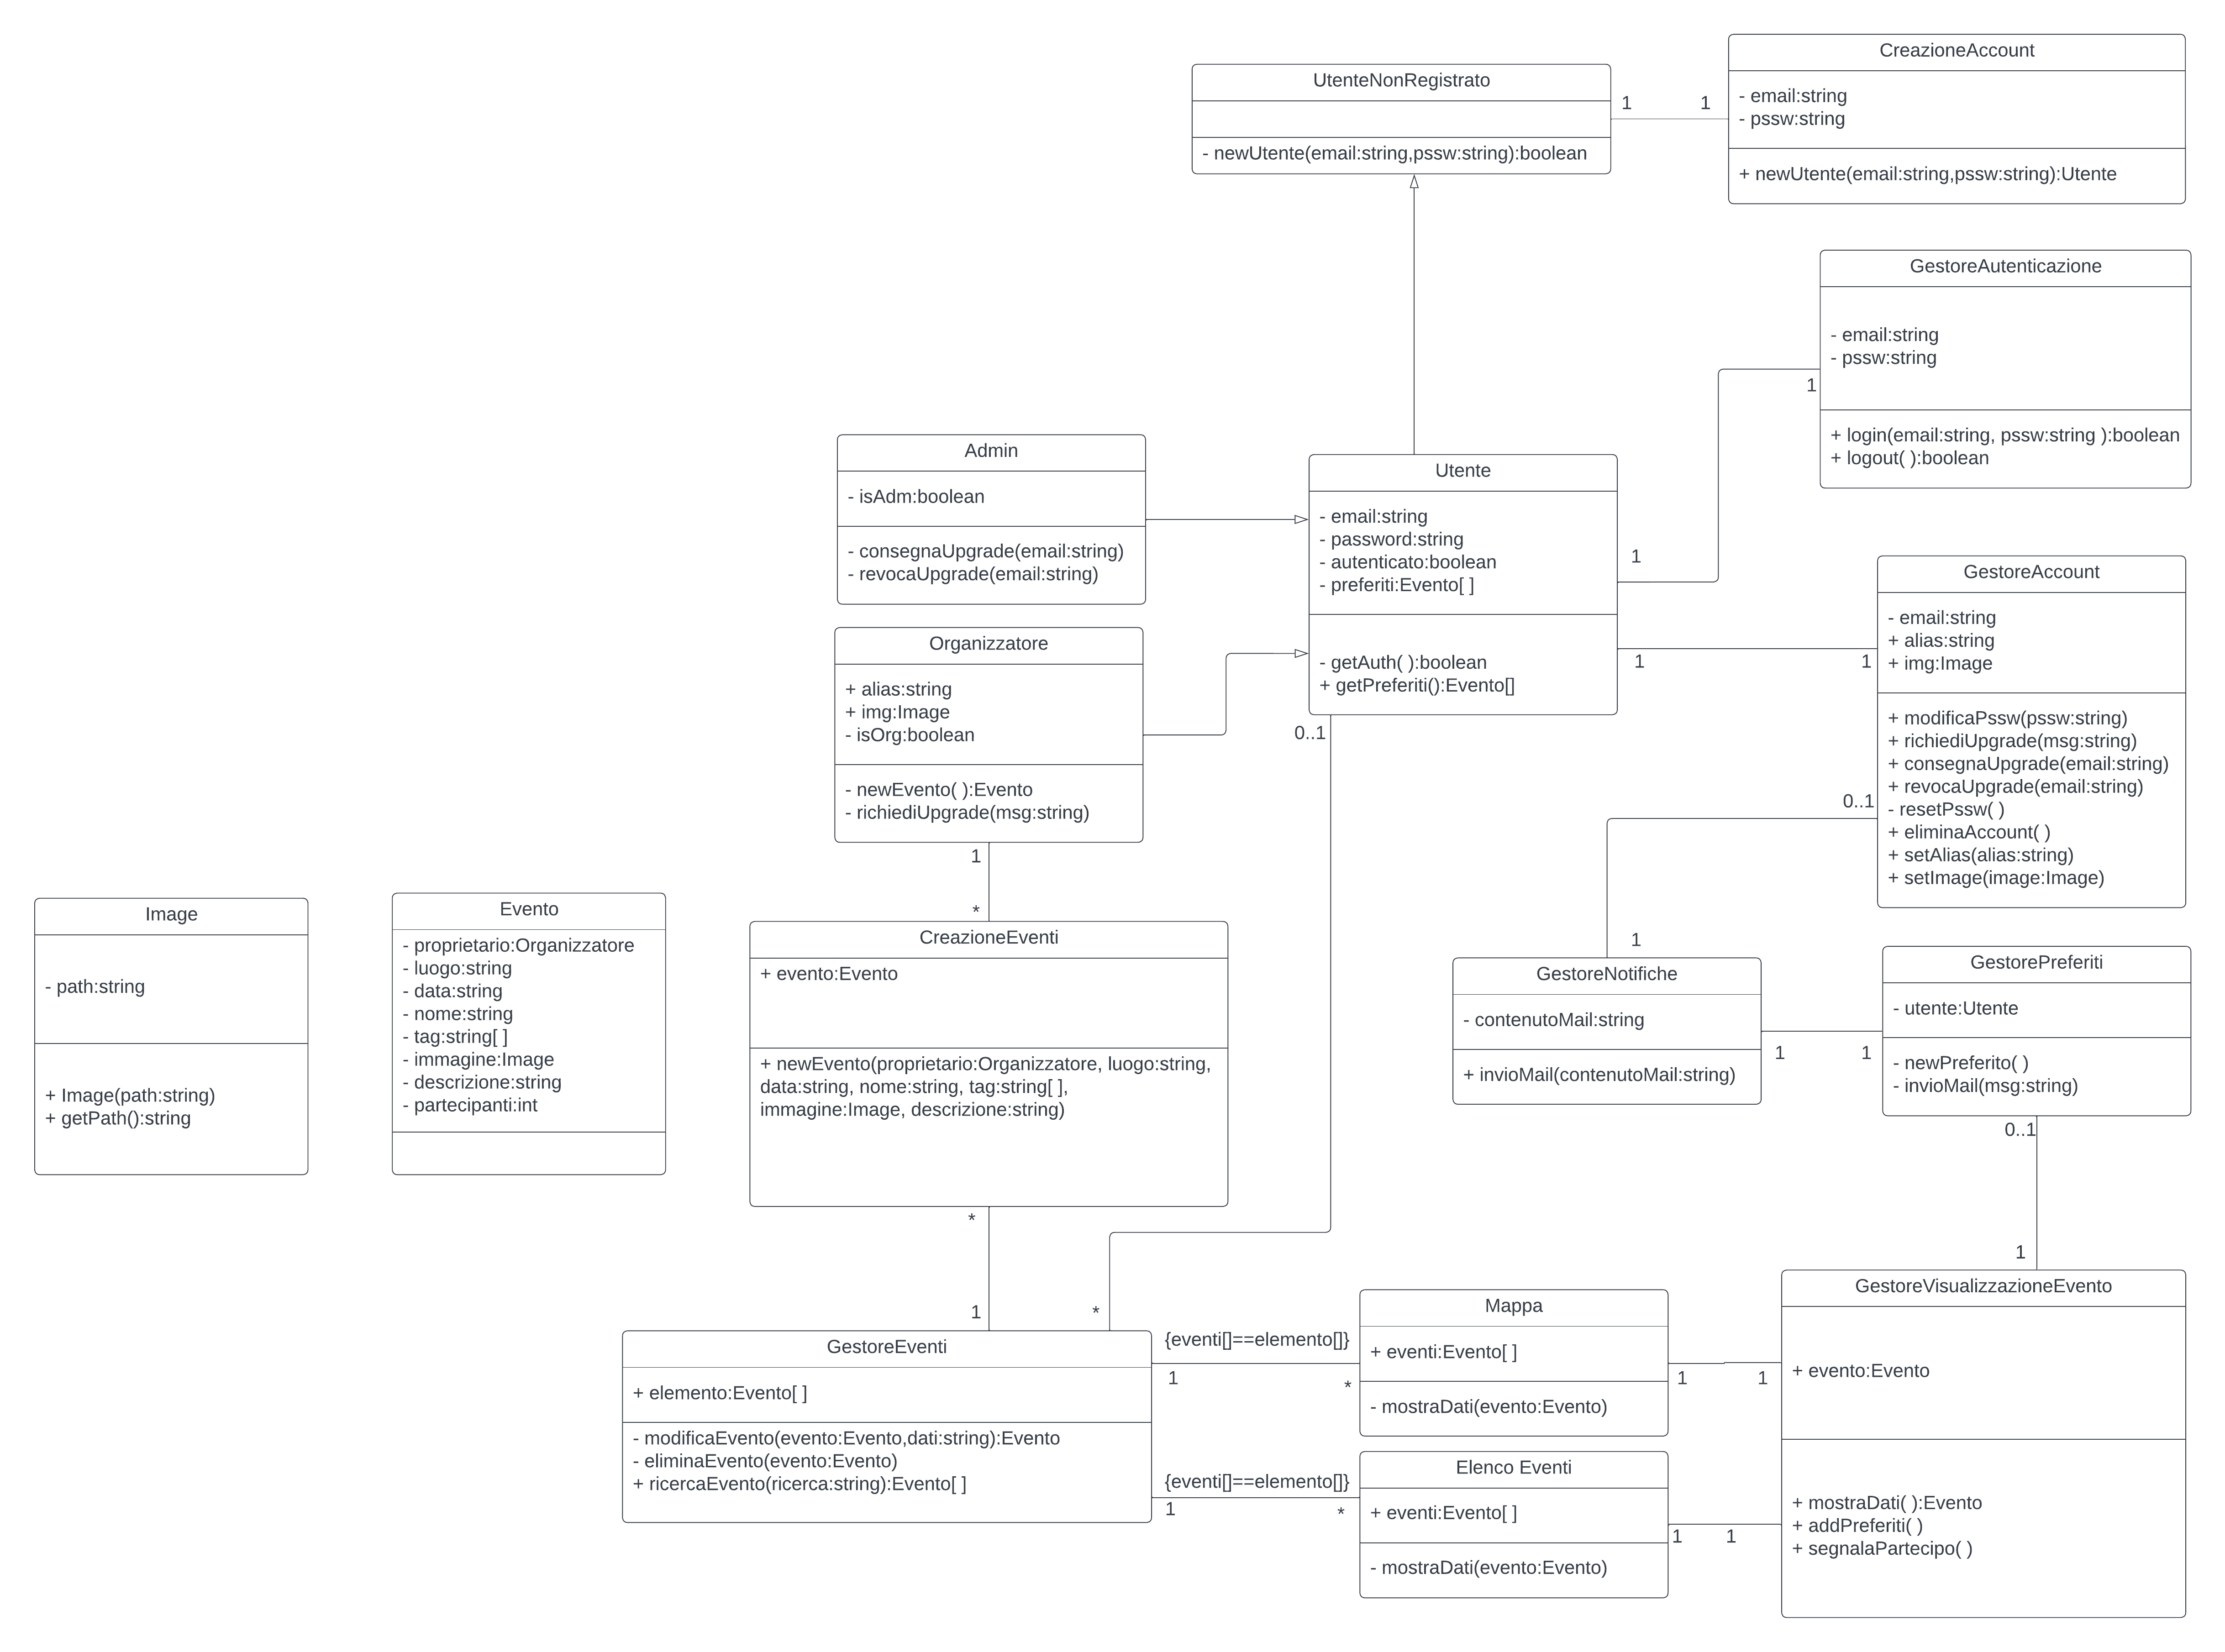
\includegraphics[scale=0.40]{class.png}
\end{center}
\clearpage
\section{Codice in Object Constraint Language}
\begin{description}
    \item[] In questo capitolo è descritta in modo formale la logica prevista nell’ambito di alcune operazioni di alcune classi. Tale logica viene descritta in Object Constraint Language (OCL).
\end{description}
\subsection{Operazioni Account Utente}
\begin{description}
    \item[] È presente una serie di restrizioni in base a se l'utente ha già effettuato il login oppure no e in base al tipo di utente. In particolare non è possibile creare un utente se ne egiste già uno con la stessa mail; la modifica della password, la richiesta di upgrade, l'eliminazione dell'account e il logout richiedono di aver già effettuato l'accesso; la richiesta di upgrade richiede inoltre che l'utente non sia già organizzatore mentre il logout cambia lo stato da autenticato a non autenticato; il reset della password e il login richiedono che l'utente non sia già autenticato (e il login cambia lo stato da non autenticato ad autenticato).
\end{description}
\begin{center}
    \item[] 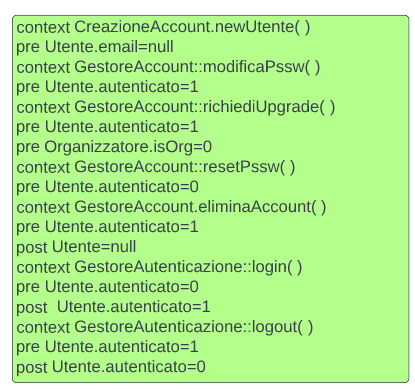
\includegraphics[scale=0.4]{oclGestoreUtenti.png}
\end{center}
\subsection{Autorizzazioni Admin}
\begin{description}
    \item[] Solo l'admin ha accesso alla consegna degli upgrade degli account e alla revoca degli stessi, previa sua autenticazione.
\end{description}
\begin{center}
    \item[] 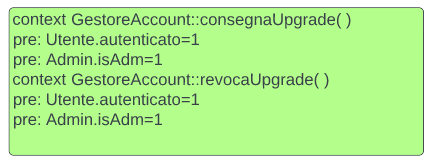
\includegraphics[scale=0.4]{oclAdmin.png}
\end{center}
\subsection{Autorizzazione Creazione Nuovo Evento}
\begin{description}
    \item[] Per poter creare un nuovo evento è necessario che l'utente sia autenticato e sia un organizzatore.
\end{description}
\begin{center}
    \item[] 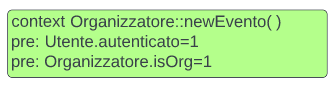
\includegraphics[scale=0.4]{oclNewEvento.png}
\end{center}
\subsection{Autorizzazioni Gestione Evento}
\begin{description}
    \item[] Per poter modificare o eliminare un evento è necessario essere admin oppure essere l'organizzatore proprietario dell'evento che si intende eliminare/modificare.
\end{description}
\begin{center}
    \item[] 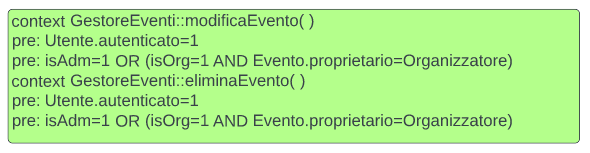
\includegraphics[scale=0.4]{oclGestioneEvento.png}
\end{center}
\subsection{Gestione Preferiti}
\begin{description}
    \item[] Il gestore preferiti permette unicamente all'utente autenticato di aggiungere un evento alla lista degli eventi preferiti se questo non è già presente e di rimuoverlo in caso contrario.
\end{description}
\begin{center}
    \item[] 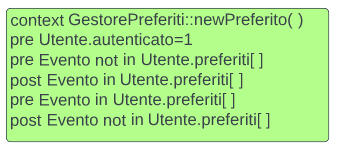
\includegraphics[scale=0.4]{oclPreferiti.png}
\end{center}
\section{Diagramma delle Classi con codice OCL}
\begin{description}
    \item[] Riportiamo infine il diagramma delle classi con tutte le classi fino ad ora presentate ed il codice OCL individuato.
\end{description}
\begin{center}
    \item[] 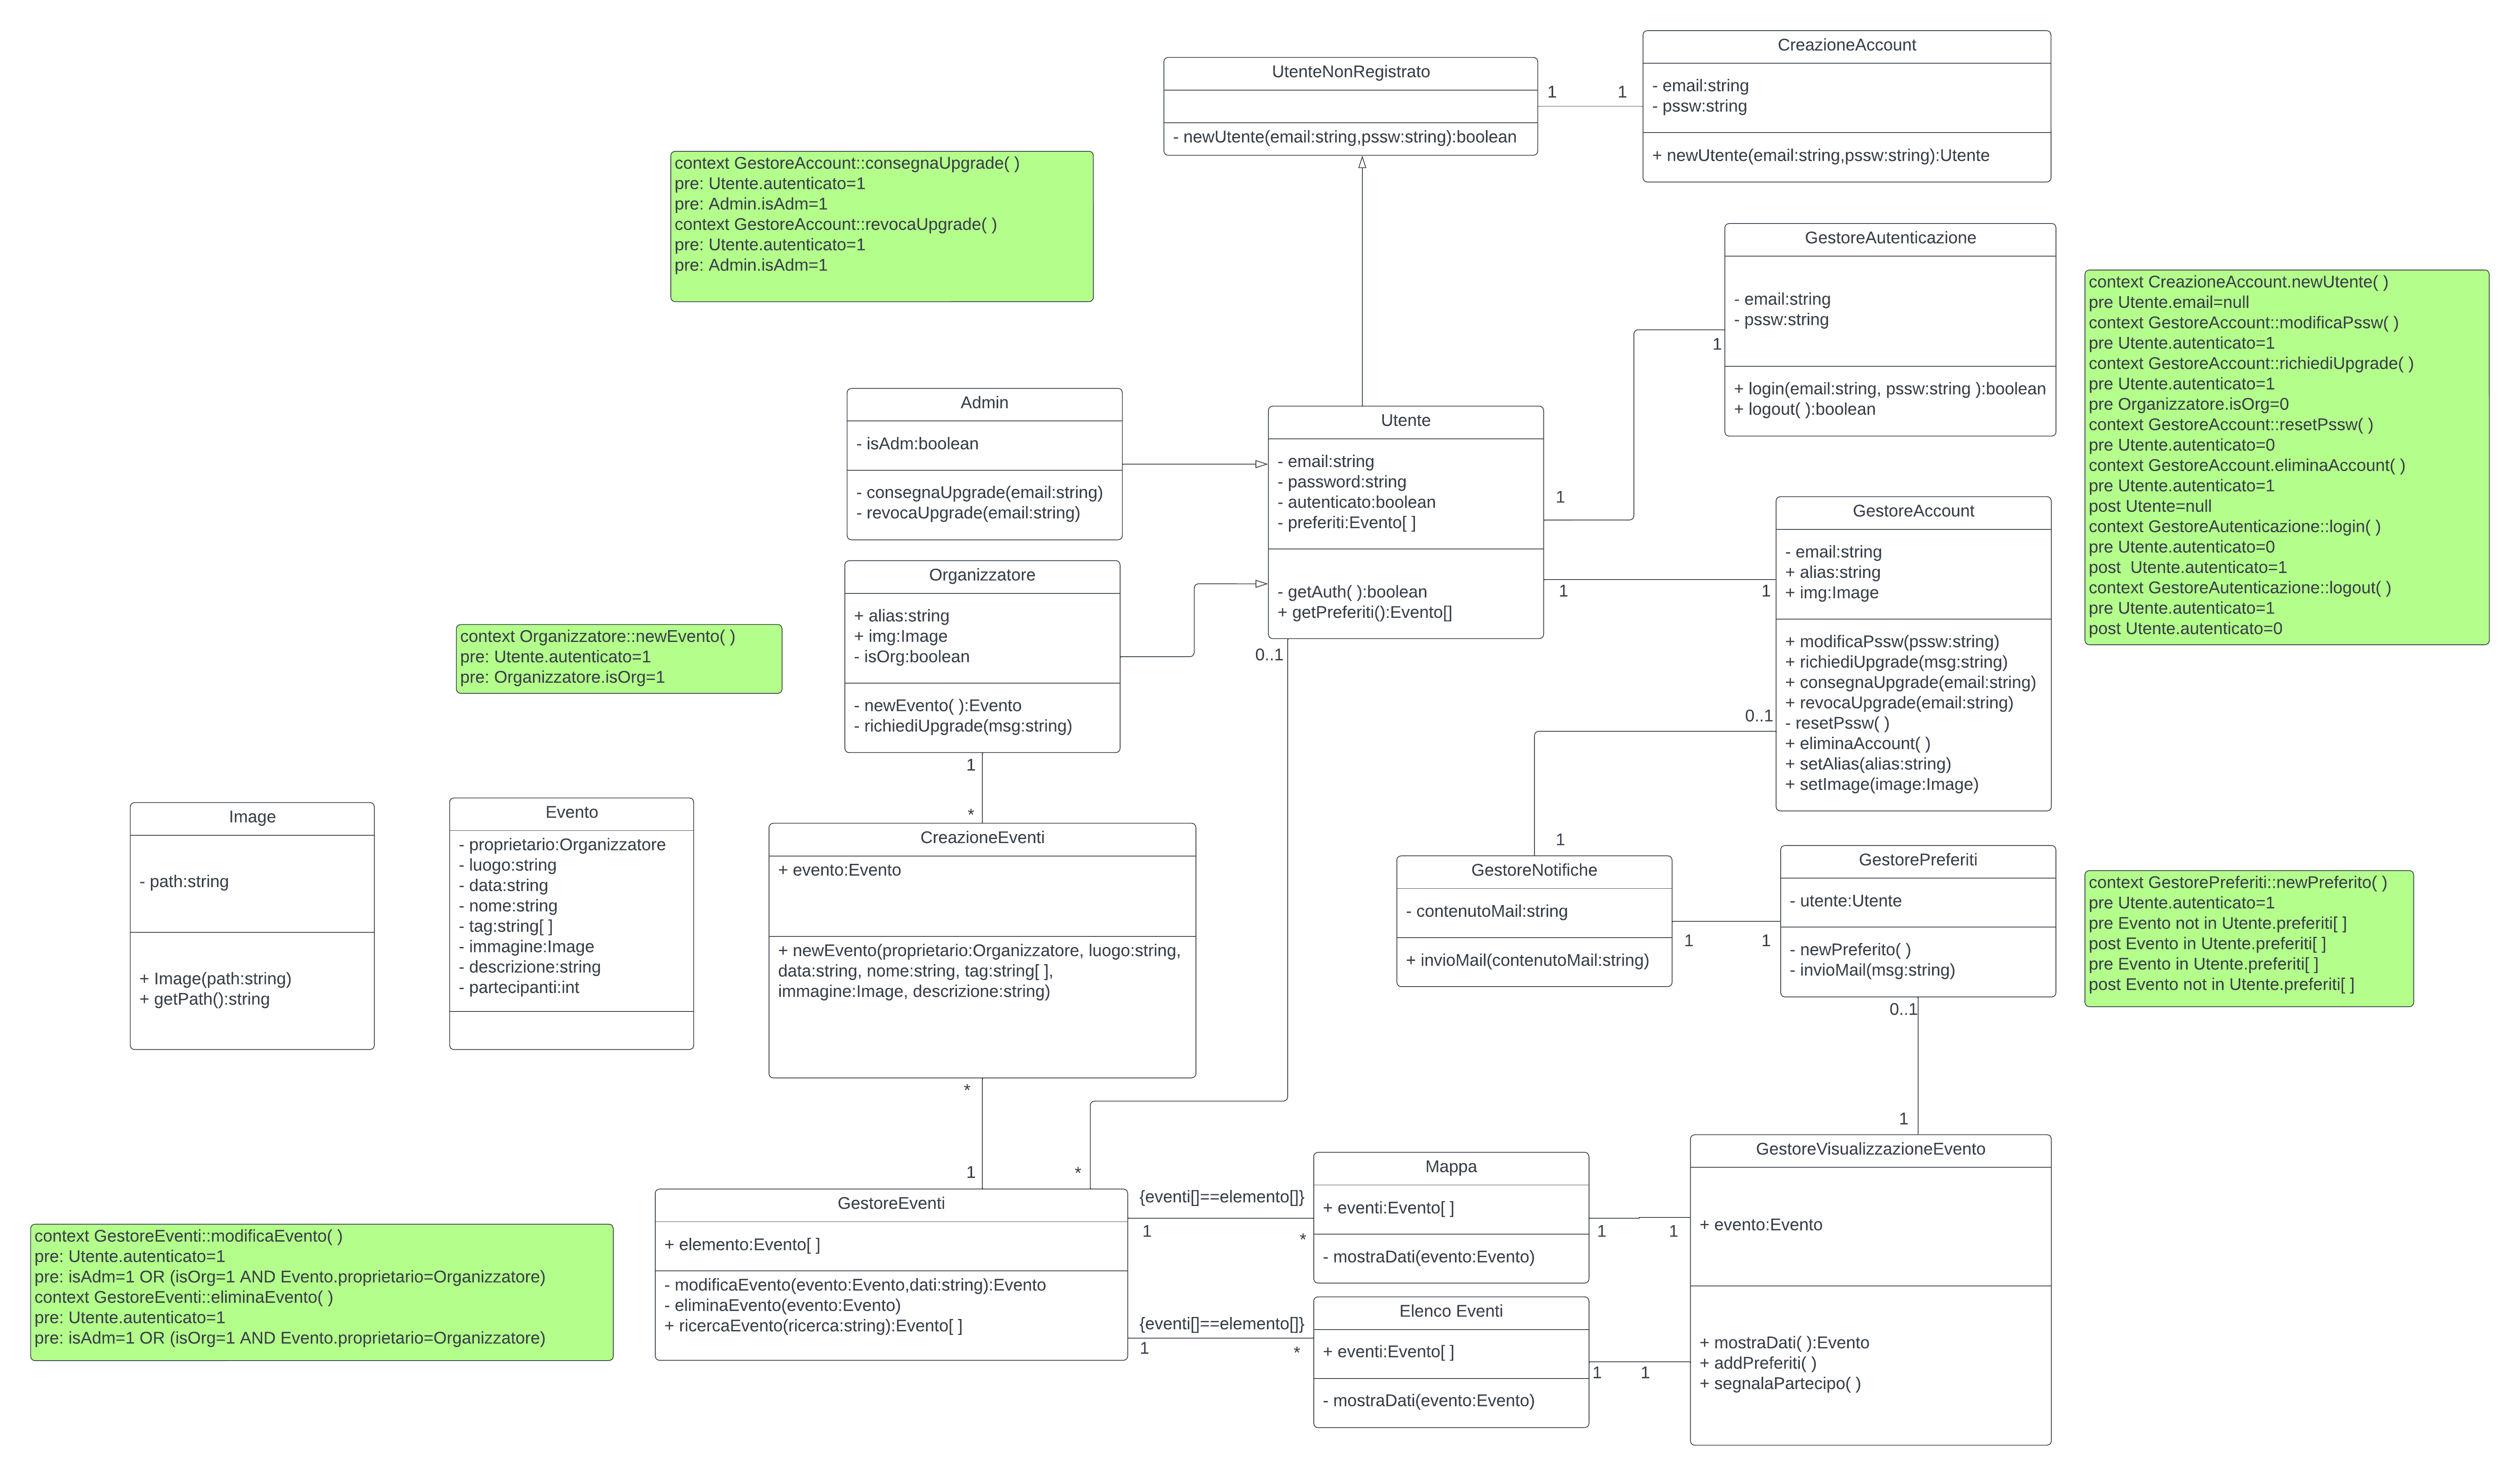
\includegraphics[scale=0.35]{oclClass.png}
\end{center}
\end{document}